
\documentclass[11pt, a4paper]{book}
\usepackage{svn-multi}
\svnid{$Id$}
\usepackage{prelim2e}
\renewcommand{\PrelimWords}{Draft Copy \svnkw{Id}}
%%\newcommand*{\mysvnrev}{\svnrev}
\usepackage[hyperindex=true,
			bookmarks=true,
            pdftitle={}, pdfauthor={Xi Yang},
            colorlinks=false,
            pdfborder=0,
            pagebackref=false,
            citecolor=blue,
            plainpages=false,
            pdfpagelabels,
            pagebackref=true,
            hyperfootnotes=false]{hyperref}
\usepackage[all]{hypcap}
\usepackage[palatino]{anuthesis}
\usepackage{afterpage}
\usepackage{graphicx}
\usepackage{thesis}
\usepackage[square]{natbib}
\usepackage[normalem]{ulem}
\usepackage[table]{xcolor}
\usepackage{makeidx}
\usepackage{cleveref}
\usepackage[centerlast]{caption2}
\usepackage{float}
\urlstyle{sf}
\renewcommand{\sfdefault}{uop}
\usepackage[T1]{fontenc}
\usepackage{bera}
\usepackage[scaled]{beramono}
\usepackage{multirow}


\renewcommand*{\backref}[1]{}
\renewcommand*{\backrefalt}[4]{
  \ifcase #1 %
    %
  \or
    (cited on page #2)%
  \else
    (cited on pages #2)%
  \fi
}



%\pdfmapfile{=fvmr8r.map}
%      $Id: macros.tex 506 2009-10-05 16:57:07Z daniel $    

\usepackage{booktabs}
\usepackage{relsize}
\usepackage{xspace}
\usepackage{subfigure}
\usepackage{listings}
\lstloadlanguages{java}
\DeclareGraphicsRule{*}{pdf}{*}{}
\newcommand{\otoprule}{\midrule[\heavyrulewidth]}
\newcommand{\pldi}{ACM Programming Language Design and Implementation (PLDI)}
\newcommand{\taco}{ACM Transactions on Architecture and Code Optimization (TACO)}
\newcommand{\lctes}{ACM Languages, Compiler, and Tool Support for Embedded Systems (LCTES)}
\newcommand{\popl}{ACM Principles of Programming Languages (POPL)}
\newcommand{\ecoop}{European Conference for Object-Oriented Programming (ECOOP)}
\newcommand{\asplos}{ACM Architectural Support for Programming Languages and Operating Systems (ASPLOS)}
\newcommand{\sigmetrics}{ACM Measurement and Modeling of Computer Systems (SIGMETRICS)}
\newcommand{\oopsla}{ACM Object-Oriented Programming, Systems, Languages, and Applications (OOPSLA)}
\newcommand{\ismm}{International Symposium on Memory Management (ISMM)}
\newcommand{\veee}{ACM/USENIX Virtual Execution Environments (VEE)}
\newcommand{\micro}{ACM/IEEE International Symposium on Microarchitecture}
\newcommand{\isca}{ACM/IEEE International Symposium on Computer Architecture (ISCA)}
\newcommand{\icse}{International Conference  on Software Engineering (ICSE)}
\newcommand{\pact}{Parallel Architectures and Compilation Techniques (PACT)}
\newcommand{\casess}{ACM Compilers, Architectures, and Synthesis for Embedded Systems (CASES)}

\definecolor{tableheadcolor}{rgb}{0.8,0.8,1.0}
%\definecolor{tablealtcolor}{rgb}{0.9,0.9,1.0}
\definecolor{tablealtcolor}{rgb}{0.9,0.9,0.95}


\definecolor{todocolor}{rgb}{0.8,0.8,1.0}
\definecolor{fixcolor}{rgb}{1,0.8,0.8}
\definecolor{commentcolor}{rgb}{0.8,1.0,0.8}


\newcommand{\listingfigure}[3]{
\begin{figure}[ht!]
  \begin{center}
    \begin{minipage}[t]{\textwidth-4cm}
      \lstinputlisting{#1}
    \end{minipage}
  \end{center}
  \caption{#3}#2
\end{figure}}

\newcommand{\includeabchart}[5]{
\begin{figure}[ht!]
\begin{center}
\newcommand{\atitle}{#4}
\newcommand{\btitle}{#5}
\input{charts/#1.tex}
\end{center}
\caption{#3}#2
\end{figure}}

\newcommand{\placeholderfigure}[2]{
\begin{figure}[ht!]
  \begin{center}
    \resizebox{\textwidth-2cm}{0.7\textwidth-1.4cm}{todo}
  \end{center}
  \caption{#2}#1
\end{figure}}

\newcommand{\singlegraphfigure}[3]{
\begin{figure}[ht!]
  \begin{center}
    \includegraphics[width=\textwidth-2cm]{#1}
  \end{center}
  \caption{#3}#2
\end{figure}}

\usepackage[color=todocolor, colorinlistoftodos]{todonotes}

%\newcommand{\notinpart}{%
% \def\toclevel@chapter{-1}\def\toclevel@section{0}\def\toclevel@subsection{1}} \newcommand{\inpart}{
% \def\toclevel@chapter{0}\def\toclevel@section{1}\def\toclevel@subsection{2}}


%
% Stuff for pretty printing the source code using listings.sty
%


%% set Java as the default language
\lstset{
  numbers=left,
  numberstyle=\tiny,
  stepnumber=1,
  numbersep=2em,
  language=java,                         % the language
  basicstyle=\footnotesize\ttfamily,     % the basic font family to use
  commentstyle=\itshape,                 % the font for comments
  stringstyle=\ttfamily,
%  morekeywords={@Intrinsic, @Unboxed, @RawStorage}
}
%\lstset{language=java}

\newcommand{\textjava}[1]{{\lstset{basicstyle=\ttfamily}\lstinline@#1@}}
\newcommand{\textjavafn}[1]{{\lstset{basicstyle=\footnotesize\ttfamily}\lstinline@#1@}}
%\usepackage{lstasm}
\usepackage{setspace}
\usepackage{ifthen}
%\usepackage{color}
%\usepackage{smallheadings}

\long\def\sfootnote[#1]#2{\begingroup%
\def\thefootnote{\fnsymbol{footnote}}\footnote[#1]{#2}\endgroup}
%
% code
%

\newcommand{\address}{\textjava{Address}\xspace}
\newcommand{\ubregion}{\textjava{unbump-region()}\xspace}
\newcommand{\word}{\textjava{Word}\xspace}
\newcommand{\freeme}{\textjava{free()}\xspace}
\newcommand{\freemeunbump}{\textjava{unbump()}\xspace}
\newcommand{\freemeunbumpregion}{\textjava{unbump-region()}\xspace}
\newcommand{\freemeunreserve}{\textjava{unreserve()}\xspace}

%
% abbreviations
%


\newcommand{\eg}{e.g., }
\newcommand{\ie}{i.e., }

\newcommand{\GenMS}{\emph{GenMS}\xspace}
\newcommand{\GenImmix}{\emph{GenIX}\xspace}
\newcommand{\mmtk}{MMTk\xspace}
\newcommand{\jikes}{Jikes RVM\xspace} 
\newcommand{\jikesrvm}{\jikes} 
\newcommand{\jala}{Jalape\~{n}o\xspace} 
\newcommand{\jalapeno}{Jalape\~{n}o\xspace} 

\newcommand{\dacapo}{\textsf{DaCapo}\xspace}
\newcommand{\specjvm}{\textsf{SPECjvm98}\xspace}
\newcommand{\cattrack}{\textsf{cattrack}\xspace}
\newcommand{\spec}{\textsf{SPEC}\xspace}

\newcommand{\nurserytype}[1]{{\fontfamily{cmss}\selectfont \textsl{#1}}}
\newcommand{\alloc}{\nurserytype{allocate}\xspace}
\newcommand{\collect}{\nurserytype{collect}\xspace}
\newcommand{\redirect}{\nurserytype{redirect}\xspace}

\newcommand{\bmtype}[1]{{\textsf{#1}}}

\newcommand{\jbb}{\bmtype{jbb2000}\xspace}
\newcommand{\psjbb}{\bmtype{pjbb2005}\xspace}
\newcommand{\pjbb}{\bmtype{pjbb2005}\xspace}
\newcommand{\specjbb}{\bmtype{SPECjbb2005}\xspace}
\newcommand{\jess}{\bmtype{jess}\xspace}
\newcommand{\raytrace}{\bmtype{raytrace}\xspace}
\newcommand{\db}{\bmtype{db}\xspace}
\newcommand{\javac}{\bmtype{javac}\xspace}
\newcommand{\jack}{\bmtype{jack}\xspace}
\newcommand{\compress}{\bmtype{compress}\xspace}
\newcommand{\mpegaudio}{\bmtype{mpegaudio}\xspace}
\newcommand{\mtrt}{\bmtype{mtrt}\xspace}
\newcommand{\antlr}{\bmtype{antlr}\xspace}
\newcommand{\bloat}{\bmtype{bloat}\xspace}
\newcommand{\chart}{\bmtype{chart}\xspace}
\newcommand{\eclipse}{\bmtype{eclipse}\xspace}
\newcommand{\fop}{\bmtype{fop}\xspace}
\newcommand{\hsqldb}{\bmtype{hsqldb}\xspace}
\newcommand{\jython}{\bmtype{jython}\xspace}
\newcommand{\luindex}{\bmtype{luindex}\xspace}
\newcommand{\lusearch}{\bmtype{lusearch}\xspace}
\newcommand{\Lusearch}{\bmtype{Lusearch}\xspace}
\newcommand{\pmd}{\bmtype{pmd}\xspace}
\newcommand{\ps}{\bmtype{ps}\xspace}
\newcommand{\SPECjbb}{\bmtype{SPECjbb}\xspace}
\newcommand{\xalan}{\bmtype{xalan}\xspace}
\newcommand{\sunflow}{\bmtype{sunflow}\xspace}
\newcommand{\Sunflow}{\bmtype{Sunflow}\xspace}
\newcommand{\avrora}{\bmtype{avrora}\xspace}
\newcommand{\core}{Core2 Quad\xspace}
\newcommand{\corelong}{Intel Core2 Quad Q6600\xspace}
\newcommand{\phenom}{Phenom II\xspace}
\newcommand{\phenomlong}{AMD Phenom II X6 1055T\xspace}
\newcommand{\sandy}{i7-2600\xspace}
\newcommand{\sandylong}{Intel Core i7-2600\xspace}



\newcommand{\ghostscript}{\bmtype{ghostscript}\xspace}

\newcommand{\doi}[1]{\href{http://dx.doi.org/#1}{\nolinkurl{doi:#1}}}
%
% misc
%
\newcommand{\fix}[1]{\todo[color=fixcolor]{#1}}
\newcommand{\comment}[1]{\todo[color=commentcolor]{#1}}
\newcommand{\ifix}[1]{\todo[inline,color=fixcolor]{#1}}
\newcommand{\icomment}[1]{\todo[inline,color=commentcolor]{#1}}
\newcommand{\itodo}[1]{\todo[inline]{#1}}
\newcommand{\ignore}[1]{}
\newcommand{\mccenter}[1]{\multicolumn{1}{c|}{#1}}

%
% figure spacing
%
%\clubpenalty 10000
%\widowpenalty 10000
%\def\topfraction{0.9}
%\def\bottomfraction{0.9}
%\def\textfraction{0.1}
%\renewcommand{\singlespacing}{\renewcommand{\baselinestretch}{1.00}\small\normalsize}
%\renewcommand{\doublespacing}{\renewcommand{\baselinestretch}{1.5}\small\normalsize}
%\newcommand{\tight}{\renewcommand{\baselinestretch}{1.28}\small\normalsize}
%\renewcommand{\subfigbottomskip}{0.25ex}
%\renewcommand{\subfigcapskip}{0ex}
%\renewcommand{\subfigcapskip}{-1ex}
%\newcommand{\subfigshrink}{-0.75ex}
%\newcommand{\subfigcapspace}{2ex}

%\newcommand{\subwidth}[0]{.32\textwidth}


%
% margins
%
%\topmargin -.5truein
%\textheight 9truein
%\oddsidemargin .25truein
%\evensidemargin .25truein
%\textwidth 6truein


%
% crossreferencing footnotes
%
%\newcommand{\fnref}[1]{~(\ref{#1})}
%\newcommand{\onecolparbox}{3.1in}


%\newcommand{\textjava}[1]{{\lstset{language=java,basicstyle=\footnotesize\ttfamily}\lstinline@#1@}}
%\newcommand{\textasm}[1]{{\lstset{language=asm,basicstyle=\footnotesize\ttfamily}\lstinline@#1@}}

%%
%% Change the sections etc.
%%
%\makeatletter
%\parskip=0pt
%\renewcommand\section{\@startsection{section}{1}{\z@}%
%                                   {-2.5ex}% beforeskip
%%                                   {1ex}% afterskip
%                                   {\large \bfseries \raggedright}}
% \renewcommand\subsection{\@startsection{subsection}{2}{\z@}%
%                                     {-2ex\@plus -1ex \@minus -.2ex}%
%                                      {.5ex \@plus .2ex}%
%                                      {\normalsize \bfseries \raggedright}}
% \renewcommand\subsubsection{\@startsection{subsubsection}{3}{\z@}%
%                                      {-2ex\@plus -1ex \@minus -.2ex}%
%                                      {1ex \@plus .2ex}%
%                                      {\normalfont\fontsize{11pt}{12pt}\selectfont\itshape}}
%\renewcommand{\thesubsubsection}{\thesubsection.\arabic{subsubsection}}

%\renewcommand\paragraph{\@startsection{paragraph}{4}{\z@}% 
%  {.5em}%
%  {-1em}%
%  {\normalfont\normalsize\bfseries\parskip=0pt}}
%\setlength\partopsep{0\p@}
%\setlength\parskip{0\p@ \@plus \p@}

%\makeatother
%\parindent=9pt





%%% Local Variables: 
%%% mode: latex
%%% TeX-master: "doa"
%%% End:

%%%%%%%%%%%%%%%%%%%%%%%%%%%%%%%%%%%%%%%%%%%%%%%%%%%%%%%%%%%%%%%%%%%%%%%
%% Preamble
\title{FaceX: A 3D Data-driven Morphable Face Synthesis Engine for Facial Expression Analysis}
\author{Xiang Li}
\date{\today}

\renewcommand{\thepage}{\roman{page}}

\makeindex
\begin{document}
%\doparttoc
%%%%%%%%%%%%%%%%%%%%%%%%%%%%%%%%%%%%%%%%%%%%%%%%%%%%%%%%%%%%%%%%%%%%%%%
%% Title page
\pagestyle{empty}
\thispagestyle{empty}
%% anuthesis.sty Copyright (C) 1996, 1997 Steve Blackburn
%% Department of Computer Science, Australian National University
%%

\begin{titlepage}
  \enlargethispage{2cm}
  \begin{center}
    \makeatletter
    \Huge\textbf{\@title} \\[.4cm]
    \Huge\textbf{\thesisqualifier} \\[2.5cm]
    \huge\textbf{\@author} \\[9cm]
    \makeatother
%%   \LARGE A thesis submitted for the degree of \\
%%    Master of Philosophy at \\
%%    The Australian National University \\[2cm]
    \LARGE A thesis submitted for the degree of \\
    Master of Machine Learning and Computer Vision \\
    The Australian National University \\[2cm]
    \thismonth
  \end{center}
\end{titlepage}


%%%%%%%%%%%%%%%%%%%%%%%%%%%%%%%%%%%%%%%%%%%%%%%%%%%%%%%%%%%%%%%%%%%%%%%
%% Here begin the preliminaries
\vspace*{14cm}
\begin{center}
  \makeatletter
  \copyright\ \@author{} 2011
  \makeatother
\end{center}
\noindent
\begin{center}
  \footnotesize{~} %\aboutthesis
\end{center}
\noindent

\newpage

\vspace*{7cm}
\begin{center}
  Except where otherwise indicated, this thesis is my own original
  work.
\end{center}

\vspace*{4cm}

\hspace{8cm}\makeatletter\@author\makeatother\par
\hspace{8cm}\today


%%%%%%%%%%%%%%%%%%%%%%%%%%%%%%%%%%%%%%%%%%%%%%%%%%%%%%%%%%%%%%%%%%%%%%%
%% Dedication
\cleardoublepage
\pagestyle{empty}
\vspace*{7cm}
\begin{center}
to my Parents,Shuanghong Li,Wenzi Liu, and my wife, Xiaorong Ma.
\end{center}


%%%%%%%%%%%%%%%%%%%%%%%%%%%%%%%%%%%%%%%%%%%%%%%%%%%%%%%%%%%%%%%%%%%%%%%
%% Acknowledgements
\cleardoublepage
\pagestyle{empty}
\chapter*{Acknowledgments}
\addcontentsline{toc}{chapter}{Acknowledgments}
First of all, I want to thank to my supervisor Tom. I was not sure at the beginning what kind of project I wanted to complete, and in what form my project was presented. Tom gave me many project options. This allowed me to choose this project when I had no idea. In the process of project development, because I am not very familiar with the field, especially unity. Tom gave me a lot of knowledge about software and project progress ideas. At the same time, I was given the channels and methods for obtaining relevant data sets. Evaluate the progress of my project through weekly meetings. At the same time, I answered the problems in my project. Secondly, I want to thank the other students in the laboratory. Actually, the progress of my project is not very smooth. I took a lot of detours and didn't find the right direction until the last few weeks. In this process, the other seniors  in the laboratory also gave me great help. Xiaoxiao will explain the content of my project so that I can go deeper into this field faster. At the same time, she answered the questions I asked patiently, even though some of them seemed very silly. I am very grateful to Xiaoxiao for helping me with this project and correcting me in time when I make detours. Other students in the laboratory also helped me a lot in this process. I am very grateful to them. Especially because of the epidemic, I can only communicate online and remotely. They always help me when I need them. Finally, I want to thank my parents and my fiancee. It was they who gave me a lot of spiritual help, and helped me ease my mood when I was depressed and stressed. At the same time, they take great care of me in life so that I can devote myself to learning.


%%%%%%%%%%%%%%%%%%%%%%%%%%%%%%%%%%%%%%%%%%%%%%%%%%%%%%%%%%%%%%%%%%%%%%%
%% Abstract
\cleardoublepage
\pagestyle{headings}
\chapter*{Abstract}
\addcontentsline{toc}{chapter}{Abstract}
\vspace{-1em}
Put your abstract here.

%%% Local Variables: 
%%% mode: latex
%%% TeX-master: "paper"
%%% End: 

%%%%%%%%%%%%%%%%%%%%%%%%%%%%%%%%%%%%%%%%%%%%%%%%%%%%%%%%%%%%%%%%%%%%%%%
%% Table of contents
\cleardoublepage
\pagestyle{headings}
\markboth{Contents}{Contents}
\tableofcontents
\listoffigures
\listoftables

%%%%%%%%%%%%%%%%%%%%%%%%%%%%%%%%%%%%%%%%%%%%%%%%%%%%%%%%%%%%%%%%%%%%%%
%% Here begins the main text
\mainmatter

%% Introduction
\chapter{Introduction}
\label{cha:intro}


\section{Thesis Statement}
\label{sec:thesisstatement}
FaceX is a lightweight, flexible and scalable engine that can be used to generate a variety of high-quality images with diversity of facial expressions and shapes. 


\section{Introduction}
\label{sec:problemstatement}
% Put your introduction here. You could use \textbackslash fix\{ABCDEFG.\} to
% leave your comments, see the box at the left side. \fix{You have to rewrite your
% thesis!!!}

In the last few decades, facial expression analysis (FEA) is a challenging task of computer vision and has attracted the interest of more and more researchers. Facial expression has been proven to play important role in understanding human emotion \citep{Mehrabian_Russell_1974}. Because facial expression is the response of a person's mental state to external stimuli \citep{Cabanac_2002}. And \citeauthor{ekmanArgumentBasicEmotions1992} classifies human emotions into seven basic categories: Happy, Sad, Surprise, Anger, Disgust, Fear and Neutral. In recent years, Compound Emtions(CEs)~\citep{duCompoundFacialExpressions2014} and Micro Expressions(MEs)~\citep{ekmanDarwinDeceptionFacial2006} have also been explored, but achievements are not rich.

With the development of artificial intelligence, especially machine learning (ML), people benefit from artificial intelligence agents adjusting their response according to their emotional state \citep{adolphsInvestigatingEmotionsFunctional2018}. In this regard, 
there are braod facial expression applications in different domains like Human-Centred Computing(Hcc) \citep{cowieEmotionRecognitionHumancomputer2001}, augmented reality (AR) \citep{chenAugmentedRealitybasedSelffacial2015}, virtual reality (VR) \citep{bekeleUnderstandingHowAdolescents2013}, automatic driving \citep{jabonFacialExpressionAnalysis2011}, and gaming \citep{lankesFacialExpressionsGame2008}. 

Various types of data can feed the FEA systems. In computer vision, facial images are the mainstream input data type. In addition, electromyography (EMG), electrocardiographic(ECG) and other related physical or chemical signal can be used as input data or auxiliary data as well \citep{jerrittaPhysiologicalSignalsBased2011}. This thesis focus on using facial images taken by sensor to detect expression and feeling of people. Because facial images contain sufficient non-verbal information for FEA \citep{huangFacialExpressionRecognition2019}. 

We briefly review the development of FEA in computer vision, most of FEA techniques can be defined as either traditional methods or learning-based methods \citep{huangFacialExpressionRecognition2019}.

\textbf{Traditional methods} involves various hand-craft features. Those approaches need to design appropriate feature extraction and choose different classifier for different dataset. Lots of conventional FEA technicals can be summarized into three main steps: preprocessing, feature extraction, facial expression classification. Preprocessing aims to reduce irrelevant redundant information and improve the ability to recognize related information. Image noise reduction, face detection and alignment and image enhancement are popular preprocessing methods. As for feature extraction, Local Binary Pattern(LBP) \citep{ahonenFaceRecognitionLocal2004}, Optical Flow \citep{hornDeterminingOpticalFlow1981}, Gabor feature \citep{lyonsCodingFacialExpressions1998}, Active Shape Model (ASM) \citep{cootesActiveShapeModelsTheir1995}, and etc. are commonly used in FEA. Another important aspect of traditional FEA methods is selecting classifier to predict facial expression. Support Vector Machine (SVM), k-Nearest Neighbours (kNN), Adaptive Boosting (Adaboost), Probabilistic Neural Network (PNN) and etc. classical ML classifier are widely deployed in FEA system. 

On the other hand,\textbf{Learning-based methods} especially for Deep-Learning (DL) have gradually become mainstream due to the great-leap-forward development of computing resources and datasets. Although the DL method outperforms and is more robust than traditional methods because it reduces the dependence on image preprocessing and hand-craft features, DL requires a huge volume of high-quality data for training compared to traditional methods. According to \citeauthor{rohSurveyDataCollection2019}, appropriate high-quality representative training data has become the bottleneck of DL. Regardless of the model, computing resources are no longer the main limitation of the end performance. Data augmentaion can alleviate the problem of insufficient data in some extent, but it is limited to the dataset itself \citep{shortenSurveyImageData2019a}. Therefore, we hope to solve this problem with pure synthetic methods. Despite the pure synthetic method greatly increases the diversity of the dataset, how to shrink the domain gap between the synthetic data set and the real data distribution is still the biggest challenge.

In this work, in order to tackle the problem of synthetic facial expression data we need to evaluates some publicly available datasets for FEA. \citep{khanSurveyAnalysisHuman2020} summarize that the facial expression dataset can be divided into video dataset and image dataset. Most public datasets only contain less than 10k images like DISFA \citep{mavadatiDISFASpontaneousFacial2013} , and some dataset less 300+ images like JAFFE \citep{lyonsCodingFacialExpressions2020}. Only a few data sets contain more than 1 million images like EmotioNet \citep{benitez-quirozEmotioNetAccurateRealTime2016a}. However, Some datasets capture a large number of images from the Internet, others are poor resolution, or the distribution of expressions is uneven. Therefore, We propose a facial expression data synthesis engine based on 3D morphable face model. This engine can synthesize a large number of labeled data with different shape, various expressions, and flexible poses. Figure \ref{fig:overview} show an overview of our engine.

\begin{figure}
    \centering
    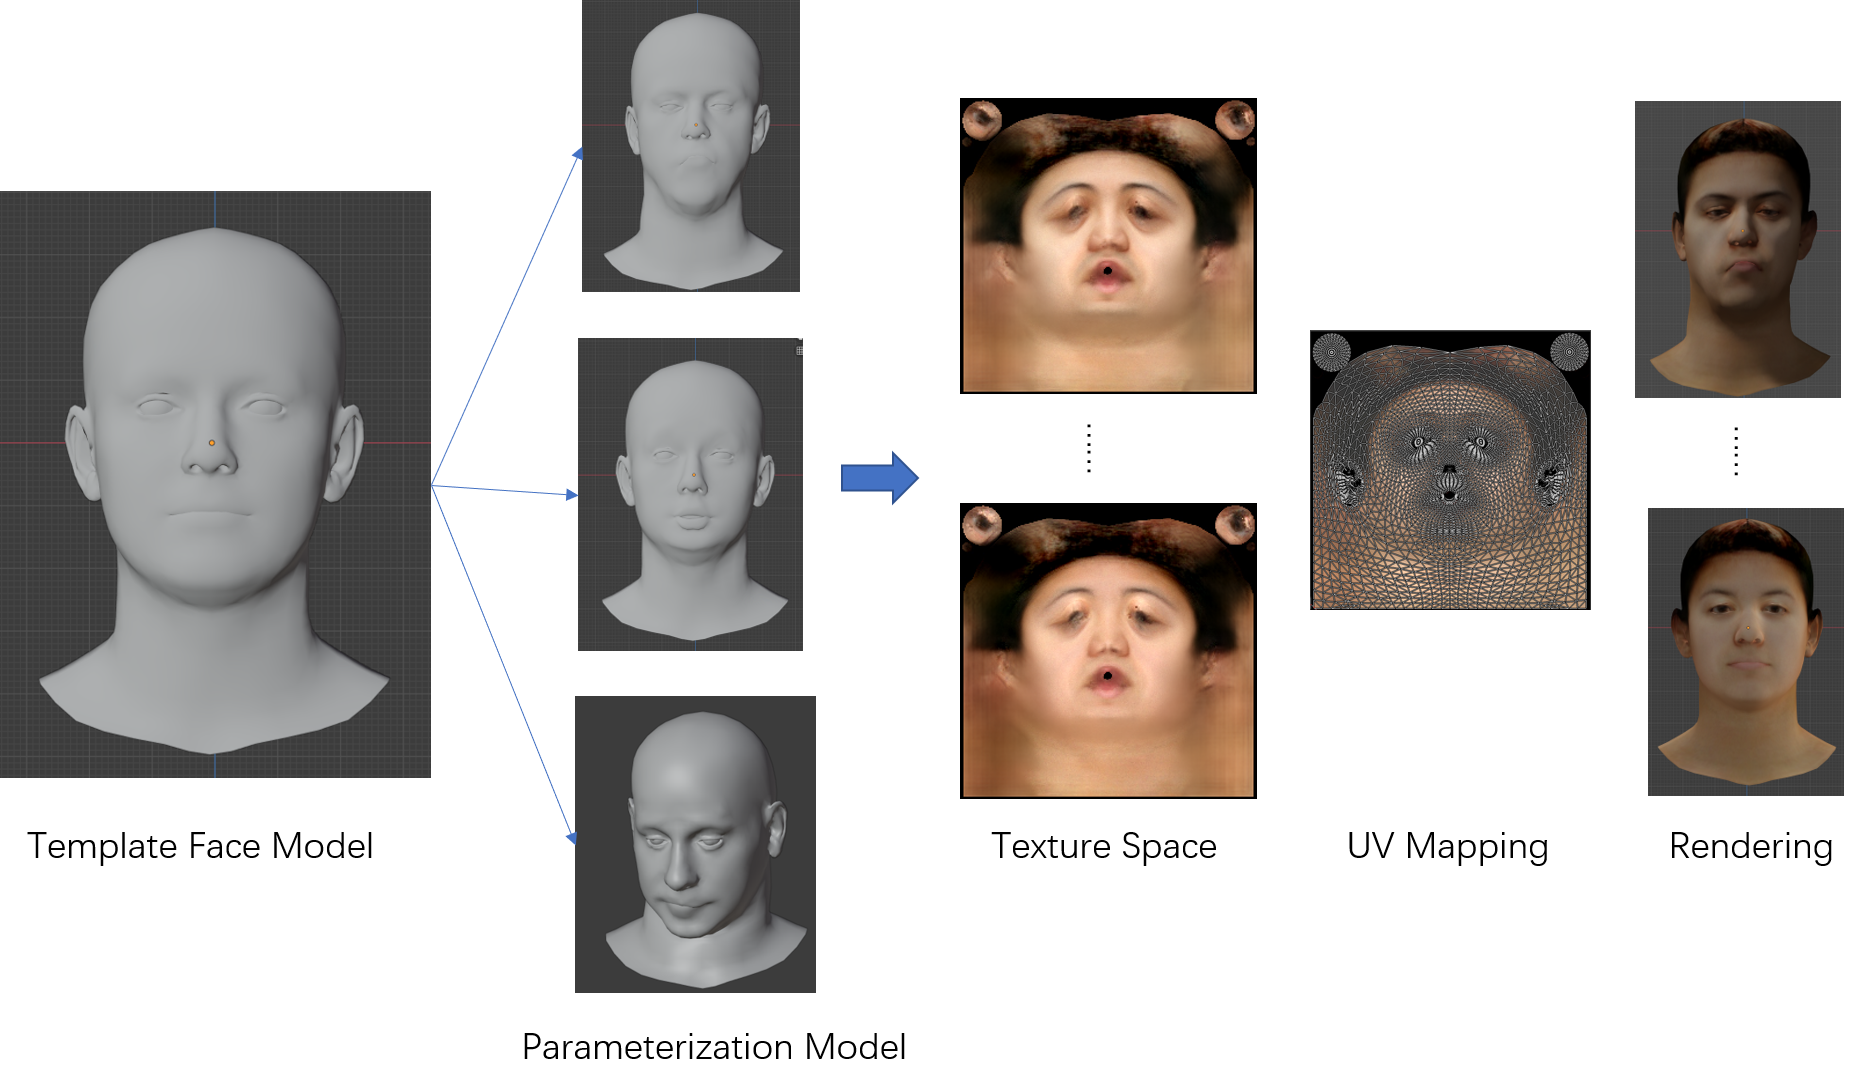
\includegraphics[width=\textwidth]{./figs/overview.png}
    \caption{Our proposed engine. We are able to generate large-scale facial expression data sets for training deep neural networks. We set the initial face model with different shape, expression and pose parameters, and sample different materials from the texture space to map to the model. Finally render under different lighting parameters.}
    \label{fig:overview}
\end{figure}
%%%%%%%%%%%%%%%%%%%%%%%%%%%%%%%%%%%%%%%%%%%%%%%%%%%%%%%%%%%%%%%%

In summary, the contributions of this thesis are as following:

\begin{itemize}
    \item Briefly summarize the development of FEA recently, and try to use synthetic data to solve the DL data bottleneck. (Section \ref{sec:problemstatement}, Chapter \ref{cha:background})
    \item Build a complete synthetic data engine, including various face shape, expression, pose and texture. (Chapter \ref{cha:design})
    \item Compare the performance of traditional FEA method with DL method on synthetic dataset. (Chapter \ref{cha:methodology})
    \item Discusse the potential problems of the synthetic data, and explain  possible improvement. (Chapter \ref{cha:conc})
\end{itemize}

\section{Thesis Outline}
\label{sec:outline}
The rest of thesis is organized from motivation to building of synthetic facial expression images.

Chapter~\ref{cha:background} introduces some details of the traditional FEA method and Learn-based method, and reviews the existing FE datasets, as well as some 3D Morphable Face Models (3DMM) that can be used for data synthesis.

Chapter~\ref{cha:design} describes the pipeline of the data synthesis engine.

Chapter~\ref{cha:methodology} is the detial of experimental design  and synthetic dataset.

Chapter~\ref{cha:result} and Chapter~\ref{cha:conc} are the results of experiments and related analytic demonstration.




%% Chapters
\chapter{Background and Related Work}
\label{cha:background}

This chapter gives a brief overview of Facial Expression Recognition,3D morphable face models and facial expression dataset. We will limit our background knowledge on discrete basic categorical model and some static based facial expression recognition techniques we used.

We widely investigated Facial Expression Recognition in Section \ref{sec:fer} at first. Then, the public available facial expression datasets are described in Section \ref{sec:fed}. Finally, we provide a review of building and applying 3D morphable face models \ref{sec:3dmm}.

\section{Facial Expression Recognition}
\label{sec:fer}
Facial expressions are the most direct and natural carrier of human emotions state\citep{darwinExpressionEmotionsMan2009}. Building an automatic facial expression analysis system has become an urgent need for artificial intelligence. In the field of computer vision and machine learning, since the early 20th century, traditional facial expression recognition  mainly benefited from the development of handcraft features and the application of classification algorithms; after 2013, due to the large number of facial expression datasets available, facial expression recognition transfers to deep learning gradually.

\subsection{Traditional methods}
Handcraft feature engineering and classification paly vital role in traditional facial expression recognition methods. In this section we will introduce several commonly used features and classifiers. The pipeline shown in Figure \ref{fig:traditional pipeline}.

\begin{figure}
    \centering
    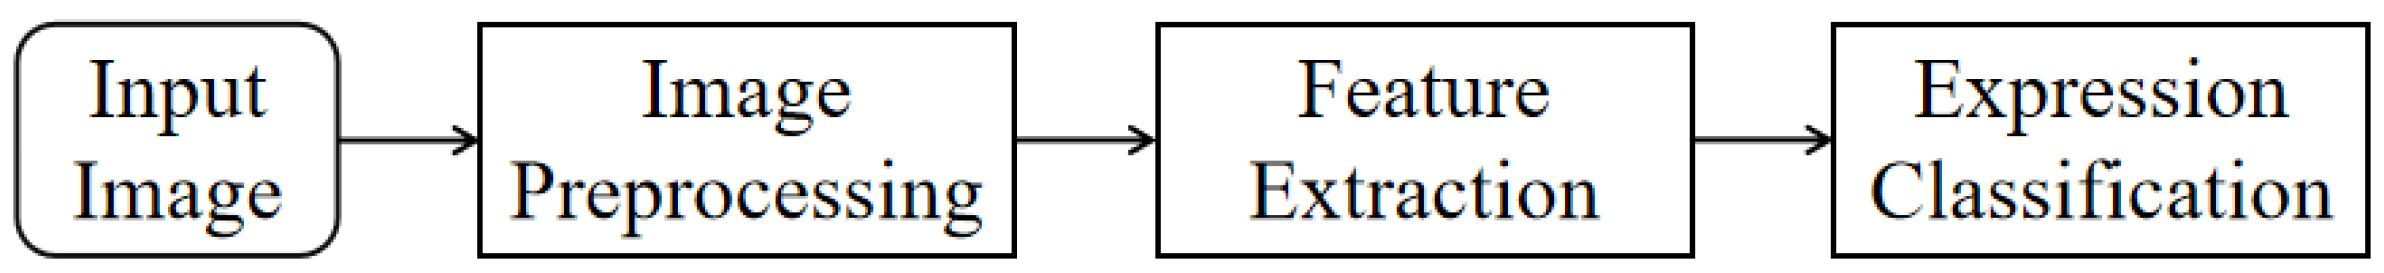
\includegraphics[width=\textwidth]{./figs/symmetry-11-01189-g004.jpg}
    \caption{\textbf{Image Processing} usually aims to reduce redundancy information of related task. \textbf{Feature Extraction} involves how to design suitable features for FEA task. \textbf{Expression Classification} is how to category features.}
    \label{fig:traditional pipeline}

\end{figure}

\subsubsection{Feature Extraction}
The purpose of feature extraction is to extract the non-pixel information expression in pixels so that the classifier can classify these features. In FER, the major used features are local binary patterns (LBP) \citep{ahonenFaceRecognitionLocal2004},Gabor feature \citep{lyonsCodingFacialExpressions1998}, and Haar-like feature \citep{violaRapidObjectDetection2001}.

\textbf{Local binary patterns (LBP):} is a simple but effective texture operator. It encodes the relationship between each pixel and nearby pixels to binary value. The most important attribute of LBP is its robustness to grayscale changes such as illumination changes. Another important feature is its computational simplicity, which enables real-time analysis of images. A simple way to encode facial expression is shown in Figure \ref{fig:LBP}.

\begin{figure}[H]
    \centering
    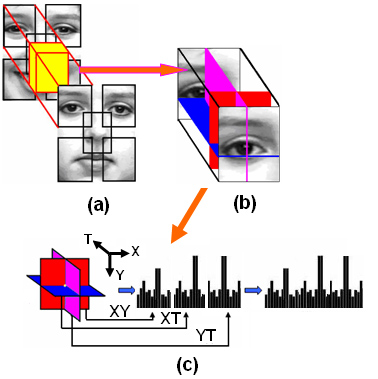
\includegraphics[width=0.5\textwidth]{./figs/LBP.jpg}
    \caption{Using LBP to encode facial expression.Divide input image into several cells, the local binary features of different cells are calculated respectively. Next, calculate the histogram of each cells. Finally, concatenate the normalized histograms to form the feature vector of input.}
    \label{fig:LBP}
\end{figure}

In the applications of FER, there are also several promoted algorithms based on LBP. For example, Complete Local Binary Pattern (CLBP)\citep{zhenhuaguoCompletedModelingLocal2010} achieves better performance than the original LBP. LBP-based Local Directional Pattern (LDP) \citep{jabidFacialExpressionRecognition2010} shows robust to illumination changes. The advantage of LBP methods is low computational complexity and small memory usage demanded. However, noise sensitivity and only focusing on local information are the disadvantages of this method.

\textbf{Gabor Feature:} is another kind of texture feature. In FER, we benefit from the multi-resolution and multi-orientation property of Gabor feature to encode facial expression image \citep{lyonsCodingFacialExpressions1998}. \citeauthor{mattelaFacialExpressionRecognition2018} proposed Gabor-mean-DWT to tackle the dimensional disaster of original Gabor feature. Gabor feature's merits is that it is not sensitive to illumination and direction, and can apply multi-scales. However, the calculation is time-consuming and requires a lot of memory.

% \textbf{Active Shape Model (ASM):} is proposed to use features to describe the geometric features of the face. The purpose is similar to face landmark detection. However, ASM is a statistical model, but face landmark detection usually uses neural network.
\textbf{Haar-like feature:} is designed to be used for target recognition tasks. It combines the lines, borders and other features of the picture. It is also the first instant face detection operation. Compared to most other features, Haar-like feature  known for calculation speed. Due to the use of integral images, any size can be calculated in constant time. However, it is sensitive to illumination. If the global region illumination diverse, the Harr-like feature may be hard to describe the local grayscale variation.


\subsubsection{Classification}
After we extract the features, another significant characteristic of the traditional method is the application of classifiers. In machine learning, the most widely used classifiers include: Support Vector Machine (SVM), k-Nearest Neighbours(kNN), Adaptive Boosting (Adaboost) and etc.

\textbf{Support Vector Machine (SVM):} aims to solve the data classification problem in the field of pattern recognition, which is a kind of supervised learning algorithm. The core of SVM is to map linearly inseparable data to a high-dimensional space through the kernel function to achieve linearly separable. Due to the characteristics of the kernel function, we can eliminate the need for complex calculations in high-dimensional space and solve the  dimension disaster to a certain extent. In FER, SVM is widely used after different features representation, and has achieved good performance \citep*{michelRealTimeFacial2003,tsaiFacialExpressionRecognition2018,hsiehEffectiveSemanticFeatures2016,saeedEmpiricalEvaluationSVM2018}.

\textbf{k-Nearest Neighbours(kNN):} is the simplest supervised classification algorithm. Typically, kNN is a representative of lazy learning due to no need for training phase. Every new data must be compared with each training data. Unfortunately, kNN has not ability to capture global structure of data. Hence, kNN might involve in local optimal solution or unstable clarification \citep*{dinoFacialExpressionClassification2019,wangNewFacialExpression2015}.

\textbf{Adaptive Boosting (Adaboost)'s:} key thought is that classifier will use the sample from last misclassified classifier  to train a classifier. AdaBoost aims to find the best training features that are useful for its weak classifiers. After each feature selection, weights will be re-adjusted by the local classification error. It reduces overfitting to a certain extent \citep*{liewFacialExpressionRecognition2015,krishnagudipatiEfficientFacialExpression2016}.

There are many other handcraft features and classifer that we have not mentioned in this section, but we can see that the major handcraft features used for facial expression recognition are geometric and texture features. This also shows that if we want to generate facial expressions data, geometry and material  will be two important components.

\subsection{Deep Learning-based Method}
% https://oysz2016.github.io/post/5d962f61.html
Compared with traditional methods, deep learning methods also have three similar steps. But it greatly reduces the model's dependence on image preprocessing and handcraft feature engineering. It also improves the robustness to the environment. In the section, we will outline the existing technologies involved in deep learning in facial expression recognition. Figure \ref{fig:deep} shows the pipeline of deep learning facial expression recognition system .
\begin{figure}[H]
    \centering
    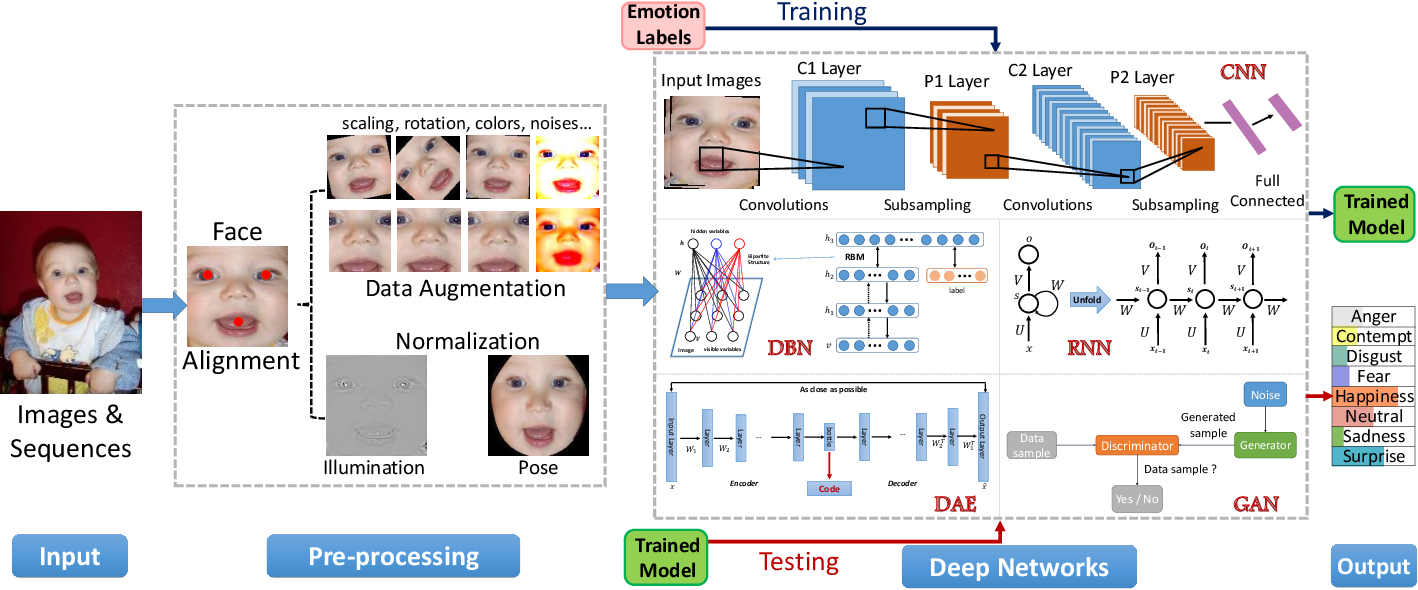
\includegraphics[width=\textwidth]{./figs/deep.png}
    \caption{A typical architecture for deep learning facial expression recognition \citep{liDeepFacialExpression2020}.}
    \label{fig:deep}
\end{figure}

\subsubsection{Image Preprocessing}
Illumination, environment and head pose changes will limit the performance of the training model. Hence, before feeding our data into deep neural network, we should normalize those visual facial semantic information as first. 

\textbf{Face alignment:} is widely used in many computer vision tasks of faces. For a given face datasets, the first step is often to detect and crop the face to eliminate irrelevant background and information.  ViolaJones(V\&J) \citep{violaRapidObjectDetection2001} is one of widely used frontal face detection, which had built in most popular computer vision library like opencv. After face detection, in order to capture the geometric features, \citeauthor{mollahosseiniGoingDeeperFacial2016} showed that with landmarks detection feeding into network, the FER performance imporve significantly. That's because it highly reduce the effect of scale and rotation of face image. Of course, many deep neural network has been employed in face detection and landmark detection. Cascaded CNN \citep{sunDeepConvolutionalNetwork2013} is the most popular technicals due to its inference speed and accuracy. Although Mutlti-task CNN \citep{zhangJointFaceDetection2016} and other multi-task network imporve the performance, we still make compromises on speed and accuracy. In our method, we use Cascaded CNN in dlib to detection face as well.

\textbf{Face normalization:} amis to reduce the effect of diversity of illumination and head pose. \textit{Illumination normalization}: Many deep learning FER system preprocess image by histogram equalization to increase the contrast \citep*{yu2015image,ebrahimi2015recurrent,pitaloka2017enhancing,10.1145/2993148.2997627}. It shows outstanding performance when the illumination normalization when the background and front face area are under near illumination condition. However, to address the overemphasizing local contrast of using histogram equalization, \citeauthor{kuo2018compact} proposed a robust histogram equalization with linear combination. And \citeauthor{pitaloka2017enhancing} measured the performance of different methods, it concluded that global contrast normalization (GCN) and histogram equalization have achieved the best performance in FER recognition. \textit{Pose normalization}: Variant head pose and occlusion significantly affect the performance of facial expression recognition system. \citeauthor{Hassner_2015} proposed using a 3D texture reference model to estimate pose, and then project back. Over the same period, \citeauthor{7410798} taken advantage of statistical model to localize landmark and estimate pose. In addition, Genrative Adversarial Network (GAN) were employed in front view synthetic and achieve better performance like DR-GAN \citep{tran2017disentangled}, TP-GAN \citep{yin2017towards}.

\subsubsection{Convolutional Neural Network (CNN)}
In computer vision and machine learning, DL has shown his capabilities of extracting low or high-level abstract features, which is more effective than handcraft features, and significantly improved performance in many fields, such as objecte detection, face recognition for identity verification and etc.. As for facial expression, Convolutional Neural Network (CNN) are widely used. \citeauthor{fasel2002robust} and \citeauthor{1167051} found that CNN has the ability to tackle pose and scala variation. It also outperformance the traditional multilayer perceptron (MLP).

AlexNet \citep{krizhevsky2017imagenet},VGG \citep{simonyan2014very},GoogleNet \citep{szegedy2015going}, Resnet \citep{he2016deep} are the most famous and popular CNN model, which has been explored in facial expression recognition. Moreover, some model proposed to address object detection task also adapt into facial expression recognition, such as Region-based CNN (R-CNN)\citep{girshick2013rich} and Faster R-CNN \citep{li2017facial}. In order to handle spatio-temporal information, 3D CNN \citep*{ji20123d,tran2014learning} has been used to capture spatial representation of expression. However, in this thesis, we only focus on static image which doesnot involve spatio-temporal feature.

% \subsubsection{Genrative Adversarial Network (GAN)}
% In recently, Genrative Adversarial Network (GAN)   
\subsubsection{Deep Learning Classification}
After learning features from model, the last step of deep learning methods also need to classify these features representation. However, unlike traditional methods, feature extraction and classification are independent of each other. In facial expression recognition, 
deep learning method can be an end-to-end approach, or just use CNN as a feature extractor and then combined with another classifier. For the first way, in CNN, the most common is to use loss function to minimize the gap between the predicted distribution and the true distribution. We can also use linear SVM \citep{tang2013deep} or other differentiable classifiers to build end-to-end facial recognition system. In addition to the end-to-end way, independent classifiers such as random forest, adaboost, and etc. can be applied to classify the extracted features from deep learning model \citep{donahue2013decaf}.



\section{Facial Expression Dataset}
\label{sec:fed}
For the design of the a deep facial expression recognition system, it is crucial to have the labeled training data. The training data are sufficient to have variations of environment as well as identify. In this section, we will introduce some public available dataset and basic information of these dataset. We will focus on their environment setting, size, drawbacks and etc..

\textbf{EmotionNet:\citep{7780969} } The dataset was released in 2017, with a total of 950,000+ images, including basic expressions, compound expressions, and face action units. With large amount of the image, this dataset cover almost all possible facial expression. All the imges were anontated by the automatic AUs detection tools. However, due to all the images are downloaded from the websites, there will not be of fixed resolution.


\textbf{AffectNet:\citep{mollahosseini2017affectnet}} The data set was released in 2017.
The dataset was collected using 1250 keywords in 6 different languages for retrieval in search engines, and get more than 42000 images. All images are labeled manually. The label type includes basic expression and realted amplitude. The expression type includes 8 basic expressions such as neutral expression, happy, sad, surprised, afraid, disgusted, angry, and contemptuous, as well as expressionless, uncertain, and unmanned. This dataset has provide annotation of searched key for all images.

\textbf{The extended CohnKanade:\citep{lucey2010complete}} This dataset was released in 2010, this database is an extension of the Cohn-Kanade Dataset, which contains 137 video frames of different facial expressions of people. CK+ contains 593 video sequence from 123 objective. The sequences has difference frames from 10 to 60. For sequences, 327 sequences from 118 subject are label with seven different facial expressions. CK+ is all in the lab. This dataset includes the frame information of the video and also gives out the peak of an expression. However, this dataset is different from the wild. When we want to use it in reality, we need to convert it.

\textbf{Aff-Wild:\citep{zafeiriou2017aff}} This dataset contains 248 videos with the length of 30 hours. All the videos in the dataset are recorded arbitrarily. It contains 130 males objects and 70 female objects. The videos are annotated by valence and arousal.Valence and arousal shows the degree of a facial expression, like degree of negative or positive. This dataset is the largest video dataset for facial expression. However due to faces are extracted from the video, numbers of subject are not high.

\textbf{Oulu-CASIA:\citep{zhao2011facial}} This dataset contains images of 80 subjects and six basic face expression, including happiness,surprise, fear, anger, sadness and disgust. National Laboratory of Pattern Recognition Beijing provides 30 Chinese sujects. University of Oulu provides 50 subjects. When they gain the dataset, they used two image light and visible light. So this dataset is popular for images which are captured in different illumination condition. However, this dataset only contains the frontal pose of subjects. 

\textbf{Denver Intensity of Spontaneous Facial Action(DISFA):\citep{mavadati2013disfa}} This data set contains videos of 27 subjects. Half are males and half are females. This dataset uses 12 action unit to encode the expression and six expression are identified including surprise, sad, smile, neutral, disgust and neural. The video in this dataset contains 4845 number of frames and also are taken based on their stimulus to an emotive video. This dataset focus on FACS standard to generate video sequence. However, this dataset does not suit for the testing staga.

\textbf{Japanese Female Facial Expression(JAFFE) Database:\citep{lyons1998coding}} The dataset was released in 1998. The database is a facial expression image captured by a camera by 10 Japanese women who made various expressions according to instructions in an experimental environment. There are a total of 213 images in the entire database, 10 people, all women, and each person makes 7 expressions. These 7 expressions are sad, happy, angry, disgusted, surprised, fearful, and neutral. There are about 20 samples in each group. Figure. Because it captured in the lab, facial expression is very clear. But the background for the image is noisy.

\textbf{MMI Facial Expression Dataset: \citep{pantic2005web} } This dataset contains over 2900 videos and high-resolution still images of 75 subjects. AUs are completely annotated. This dataset is laboratory-controlled. The 213 sequence are labeled with six basic expression. The sequence in this dataset are onset-apex-offset labeled.

\textbf{Binghamton University 3D Facial Expression(BU-3DFE): \citep{yin20063d}} This dataset is designed for research on 3D facial expression. It contains 56 females and 44 males subject and 100 in total. Those subjects are from various racial ancestries. Also they have wide age range from 18 to 70. This dataset contains six basic facial expressions. Also, 3D facial models for each sbuject are introduced in the dataset. Also 83 manually annotated facial landmark connected with each model are contained. This dataset is used for multiview 3D facial expression analysis.

\textbf{FER2013 Face Dataset : \citep{carrier2013fer}} This dataset was released in 2013. This dataset contains 35887 face images and includes 28709 training sets, and 3589 verification sets and 589 test sets. All the images are gray scale with 48 pixels plus 48 pixels. This dataset contains seven basic face expressions incluidng fear, anger, sad, surprise, happy, disgust and neutral. Each sample in the dataset has a wide range of age, direction. So it is closed to the real world.

\textbf{ Real-word Affective Database(RAF-DB) : \citep{li2018reliable}} This dataset contains 29672 diverse facial images. All the images are downloade from the website. This dataset contains six basic and eleven compound emotion. The 15339 images from the basic emotion set were separated into two group, including training sample and test sample.

% We summarize the information of different facial expression dataset. 

Among these dataset, we can summarize that images from those larger size facial expression datasets are variant resolution, even most of data are low resolution, and inconsistency among different image quality. On the other hand, images from those larger size facial expression datasets are usually generated in the laboratory condition. Therefore, those dataset lack the diversity. In this condition, we aim to solve the quailty of the facial expression image and the diversity of the data images.

% So I am trying to make use of the unity, blender, Maya and other 3D modeling software to achieve synthetic face data.

\section{3D Morphable Face Models}
\label{sec:3dmm}
One of the most typical ways to synthesize data is to use game engines, such as Unity, Unreal, or modeling tools like Blender, C3D to synthesize data in the virtual physical world.

When we use the 3D engine to synthetic data, we need to find out or construct suitable morphable facial model. Thus, in this section we will investigate 3D Morphable Face Models (3DMM).

A 3D morphable face model is a genertive model for face shape and appearance. 3D Morphable Face Models were first introduced in 1999\citep{blanz1999morphable}. And these models were used as a general principled approach to analyse images. There are different ways to compute a 3DMM by modeling. In this part, I will introduce these three different ways.

\subsection{Shape model}

The Shape model is classical modeling approach that uses 3D data. A shape space is traditionally defined as the set of all configuration of $n$ vertices in 3D space with fixed connectivity\citep{dryden2016statistical}. Commonly used model are two models. One is the global model that represents variation of the entire face surface. The other is the local model that varation of facial parts.


\subsection{Expression model}

This kind of model captures variation of both identity and expression. Unlike simple linear models which learn through a dataset that has different identity and expression, this model focus on explicitly decouple the influence of identity and expression\citep{booth20173d}. This is achieve by modeling in separate coefficients. 

There are three different kinds of methods. The first one is additive model. This model gives two shape of the subject,including expression and neutral shape. It tranferred expression between subject by adding the offset of the expression\citep{blanz1999morphable}. The second is multiplicative model. A common multiplicative model is the concept of the multilinear model, which extends the idea that PCA performs singular value decomposition. The decomposition of the 3D face data into a stack of training data (HOSVD) by performing higher order tensor data to tensor data\citep{vlasic2006face}. The third is nonlinear model. There also some methods to model facial variation with nonlinear transformation, such as FLAME, an articulated expressive head model that gives nonlinear control\cite{yu2017learning}.

\subsection{Appearance model}

The appearance model is to capture variation in appearance and illumination. The most common way to build it is to provide statistics on the appearance of the training shape, where the appearance information is usually expressed as a value per vertex or as a texture in the uv space\citep{booth20173d}. There are two models. One is the linear per-vetex model which is low-dimension texture, the other is linear texture space model which require compatible resolution.

\subsection{Public Available 3D Morphable Facial Model}

\textbf{Base Face Model(BFM) 2009 : \citep{paysan20093d}} This model is a kind of the shape model. Pascal Paysan used a laser scanner to accurately collect 200 individual data in 2009 to obtain the Basel Face Model dataset. The entire data set contains 200 three-dimensional faces. Among them, 100 were males and 100 were females, and most of them were Caucasian. The age distribution of these data is 8 to 62 years old. Everyone was collected 3 neutral expressions and selected the most natural one.

\textbf{FaceWarehouse : \citep{cao2013facewarehouse}} This model is kind of shape and expression model. Cao used Kinect's RGBD camera to capture 150 individuals from 7-80 years old from different ethnic backgrounds. For each person, it collected RGBD data of her different expressions, including neutral expressions and 19 other expressions.
FaceWareHouse is widely used in visualization calculations, especially the bilinear face model has excellent performance in estimating face identity and expression in pictures and videos.

\textbf{Surrey Face Model: \citep{huber2016multiresolution}} This model is kind of shape abd expression model. This model is a multi-resolution 3D deformed face model provided by the University of Surrey in the UK.The model contains different grid resolution levels and landmark point annotations, as well as metadata for texture remapping.

\textbf{Face Learned with an Articulated Model and expression(FLAME) : \citep{yu2017learning}} This is kind of shape, expression and head pose model. It contains 3800 individualis for shape, 800 for head pose and 21000 frames for expression. It considers different genders and also a full head model without hair.

\textbf{Base Face Model(BFM) 2017: \citep{gerig2018morphable}} This is kind of shape and expression model. It has 200 individuals for shape and appearance and a total of 160 expression scans. Also this is an extension of the BFM 2009. Compare with the BFM 2009, BFM 2019 has multiresolution and was with full head. 

\textbf{Morphable Face Albedo Model:\citep{smith2020morphable} }
This model is an extension of BFM 2017. It contains 73 individuals.The model captured data to provide ground truth for an albedo estimation benchmark using the same fitting pipeline. This model reduces the error in the estimated albedo by nearly 70 percent compared to using the existing base face model


\section{Summary}
In this chapter, we first introduce the traditional methods for FEA. We found that the design features of traditional methods are mainly focused on the geometric features and texture features of the face. This inspired us that for synthesize facial expression data, we should not only pay attention to the geometry information, such as the outline of the face. The material also contains the underlying information of the facial expression.

Moreover, we compared deep learning with traditional methods and summarized the application of deep learning in facial expression recognition. 

Finally, we summarized the public facial expression dataset and 3d Morphable face models, and explained their potential problems and advantages.

% Summary what you discussed in this chapter, and mention the story in next
% chapter. Readers should roughly understand what your thesis takes about by only reading
% words at the beginning and the end (Summary) of each chapter.




\chapter{Synthetic Data Generation}
\label{cha:design}
Same as the last chapter, introduce the motivation and the high-level picture to
readers, and introduce the sections in this chapter.


\section{Face Model}
\label{sec:face}

\section{Expression Model}
\label{sec:expression}


\section{Texture Model}
\label{sec:texture}

\section{Data Generation}
\label{sec:data_generation}
\chapter{Experiment and Result}
\label{cha:methodology}

\section{Dataset}
\label{sec:softplat}
\subsection{Dataset for training expression parameters}
\subsection{Pure Synthetic data}
12000 images,7 different expression, 2000 subject.

\section{Evaluation}
\label{sec:hardplat}
\subsection{Face landmarks + HOG with SVM}
\subsection{Different CNN scheme}
\begin{itemize}
  \item Baseline simple CNN
  \item ResNet FER
\end{itemize}



\section{Example of synthetic facial image}


\section{Results}




%%% Local Variables: 
%%% mode: latex
%%% TeX-master: "paper"
%%% End: 

\chapter{Results}
\label{cha:result}

\section{Direct Cost}\
\label{sec:direct_cost}

Here is the example to show how to include a figure. Figure~\ref{fig:cost}
includes two subfigures (Figure~\ref{fig:zerocost}, and Figure~\ref{fig:zerobus});

\begin{figure*}
  \label{fig:cost}
  \subfigure[Fraction of cycles spent on zeroing\label{fig:zerocost}]{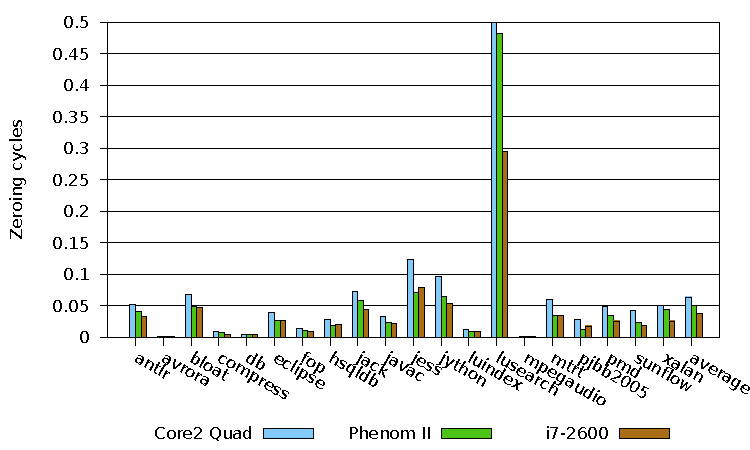
\includegraphics[width=\columnwidth]{figs/zerocost_intel.pdf}}
  \subfigure[BytesZeroed / BytesBurstTransactionsTransferred\label{fig:zerobus}]{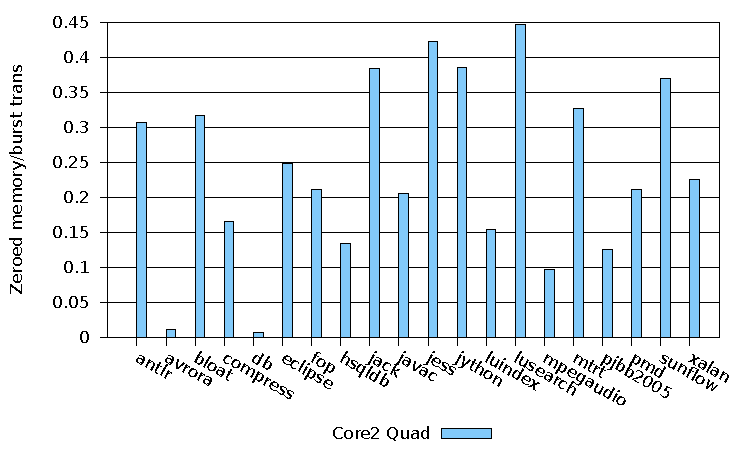
\includegraphics[width=1.0\columnwidth]{figs/zerobus_core.pdf}}
  \caption{The cost of zero initialization}
\end{figure*}


\section{Summary}

\chapter{Conclusion}
\label{cha:conc}
Summary your thesis and discuss what you are going to do in the future in Section~\ref{sec:future}.


\section{Future Work}
\label{sec:future}
Good luck.





%%%%%%%%%%%%%%%%%%%%%%%%%%%%%%%%%%%%%%%%%%%%%%%%%%%%%%%%%%%%%%%%%%%%%%
% Here begins the end matter

%%% \appendix

\backmatter

\bibliographystyle{anuthesis}
\bibliography{thesis}

\printindex

\end{document}
